% Created by tikzDevice version 0.12.3.2 on 2022-02-17 23:06:06
% !TEX encoding = UTF-8 Unicode
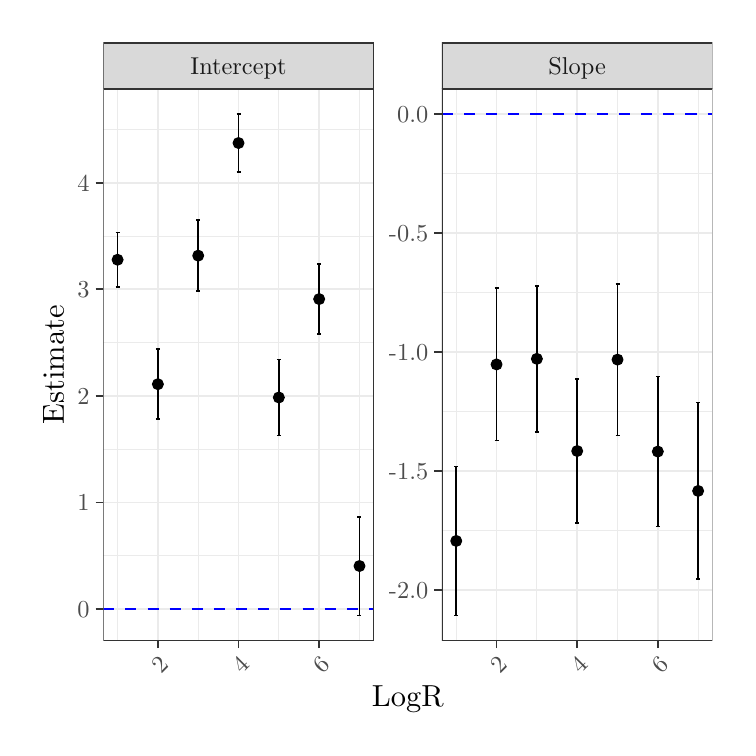
\begin{tikzpicture}[x=1pt,y=1pt]
\definecolor{fillColor}{RGB}{255,255,255}
\path[use as bounding box,fill=fillColor,fill opacity=0.00] (0,0) rectangle (252.94,252.94);
\begin{scope}
\path[clip] (  0.00,  0.00) rectangle (252.94,252.94);
\definecolor{drawColor}{RGB}{255,255,255}
\definecolor{fillColor}{RGB}{255,255,255}

\path[draw=drawColor,line width= 0.6pt,line join=round,line cap=round,fill=fillColor] (  0.00,  0.00) rectangle (252.94,252.94);
\end{scope}
\begin{scope}
\path[clip] ( 27.31, 31.52) rectangle (125.07,230.87);
\definecolor{fillColor}{RGB}{255,255,255}

\path[fill=fillColor] ( 27.31, 31.52) rectangle (125.07,230.87);
\definecolor{drawColor}{gray}{0.92}

\path[draw=drawColor,line width= 0.3pt,line join=round] ( 27.31, 62.09) --
	(125.07, 62.09);

\path[draw=drawColor,line width= 0.3pt,line join=round] ( 27.31,100.61) --
	(125.07,100.61);

\path[draw=drawColor,line width= 0.3pt,line join=round] ( 27.31,139.13) --
	(125.07,139.13);

\path[draw=drawColor,line width= 0.3pt,line join=round] ( 27.31,177.65) --
	(125.07,177.65);

\path[draw=drawColor,line width= 0.3pt,line join=round] ( 27.31,216.17) --
	(125.07,216.17);

\path[draw=drawColor,line width= 0.3pt,line join=round] ( 32.49, 31.52) --
	( 32.49,230.87);

\path[draw=drawColor,line width= 0.3pt,line join=round] ( 61.62, 31.52) --
	( 61.62,230.87);

\path[draw=drawColor,line width= 0.3pt,line join=round] ( 90.76, 31.52) --
	( 90.76,230.87);

\path[draw=drawColor,line width= 0.3pt,line join=round] (119.90, 31.52) --
	(119.90,230.87);

\path[draw=drawColor,line width= 0.6pt,line join=round] ( 27.31, 42.83) --
	(125.07, 42.83);

\path[draw=drawColor,line width= 0.6pt,line join=round] ( 27.31, 81.35) --
	(125.07, 81.35);

\path[draw=drawColor,line width= 0.6pt,line join=round] ( 27.31,119.87) --
	(125.07,119.87);

\path[draw=drawColor,line width= 0.6pt,line join=round] ( 27.31,158.39) --
	(125.07,158.39);

\path[draw=drawColor,line width= 0.6pt,line join=round] ( 27.31,196.91) --
	(125.07,196.91);

\path[draw=drawColor,line width= 0.6pt,line join=round] ( 47.05, 31.52) --
	( 47.05,230.87);

\path[draw=drawColor,line width= 0.6pt,line join=round] ( 76.19, 31.52) --
	( 76.19,230.87);

\path[draw=drawColor,line width= 0.6pt,line join=round] (105.33, 31.52) --
	(105.33,230.87);
\definecolor{drawColor}{RGB}{0,0,255}

\path[draw=drawColor,line width= 0.6pt,dash pattern=on 4pt off 4pt ,line join=round] ( 27.31, 42.83) -- (125.07, 42.83);
\definecolor{drawColor}{RGB}{0,0,0}
\definecolor{fillColor}{RGB}{0,0,0}

\path[draw=drawColor,line width= 0.4pt,line join=round,line cap=round,fill=fillColor] ( 32.49,169.08) circle (  1.96);

\path[draw=drawColor,line width= 0.4pt,line join=round,line cap=round,fill=fillColor] ( 47.05,124.11) circle (  1.96);

\path[draw=drawColor,line width= 0.4pt,line join=round,line cap=round,fill=fillColor] ( 61.62,170.56) circle (  1.96);

\path[draw=drawColor,line width= 0.4pt,line join=round,line cap=round,fill=fillColor] ( 76.19,211.25) circle (  1.96);

\path[draw=drawColor,line width= 0.4pt,line join=round,line cap=round,fill=fillColor] ( 90.76,119.31) circle (  1.96);

\path[draw=drawColor,line width= 0.4pt,line join=round,line cap=round,fill=fillColor] (105.33,154.87) circle (  1.96);

\path[draw=drawColor,line width= 0.4pt,line join=round,line cap=round,fill=fillColor] (119.90, 58.41) circle (  1.96);

\path[draw=drawColor,line width= 0.6pt,line join=round] ( 31.76,178.97) --
	( 33.21,178.97);

\path[draw=drawColor,line width= 0.6pt,line join=round] ( 32.49,178.97) --
	( 32.49,159.19);

\path[draw=drawColor,line width= 0.6pt,line join=round] ( 31.76,159.19) --
	( 33.21,159.19);

\path[draw=drawColor,line width= 0.6pt,line join=round] ( 46.32,136.71) --
	( 47.78,136.71);

\path[draw=drawColor,line width= 0.6pt,line join=round] ( 47.05,136.71) --
	( 47.05,111.50);

\path[draw=drawColor,line width= 0.6pt,line join=round] ( 46.32,111.50) --
	( 47.78,111.50);

\path[draw=drawColor,line width= 0.6pt,line join=round] ( 60.89,183.40) --
	( 62.35,183.40);

\path[draw=drawColor,line width= 0.6pt,line join=round] ( 61.62,183.40) --
	( 61.62,157.72);

\path[draw=drawColor,line width= 0.6pt,line join=round] ( 60.89,157.72) --
	( 62.35,157.72);

\path[draw=drawColor,line width= 0.6pt,line join=round] ( 75.46,221.81) --
	( 76.92,221.81);

\path[draw=drawColor,line width= 0.6pt,line join=round] ( 76.19,221.81) --
	( 76.19,200.69);

\path[draw=drawColor,line width= 0.6pt,line join=round] ( 75.46,200.69) --
	( 76.92,200.69);

\path[draw=drawColor,line width= 0.6pt,line join=round] ( 90.03,133.08) --
	( 91.49,133.08);

\path[draw=drawColor,line width= 0.6pt,line join=round] ( 90.76,133.08) --
	( 90.76,105.54);

\path[draw=drawColor,line width= 0.6pt,line join=round] ( 90.03,105.54) --
	( 91.49,105.54);

\path[draw=drawColor,line width= 0.6pt,line join=round] (104.60,167.58) --
	(106.06,167.58);

\path[draw=drawColor,line width= 0.6pt,line join=round] (105.33,167.58) --
	(105.33,142.17);

\path[draw=drawColor,line width= 0.6pt,line join=round] (104.60,142.17) --
	(106.06,142.17);

\path[draw=drawColor,line width= 0.6pt,line join=round] (119.17, 76.23) --
	(120.62, 76.23);

\path[draw=drawColor,line width= 0.6pt,line join=round] (119.90, 76.23) --
	(119.90, 40.58);

\path[draw=drawColor,line width= 0.6pt,line join=round] (119.17, 40.58) --
	(120.62, 40.58);
\definecolor{drawColor}{gray}{0.20}

\path[draw=drawColor,line width= 0.6pt,line join=round,line cap=round] ( 27.31, 31.52) rectangle (125.07,230.87);
\end{scope}
\begin{scope}
\path[clip] (149.69, 31.52) rectangle (247.44,230.87);
\definecolor{fillColor}{RGB}{255,255,255}

\path[fill=fillColor] (149.69, 31.52) rectangle (247.44,230.87);
\definecolor{drawColor}{gray}{0.92}

\path[draw=drawColor,line width= 0.3pt,line join=round] (149.69, 71.23) --
	(247.44, 71.23);

\path[draw=drawColor,line width= 0.3pt,line join=round] (149.69,114.25) --
	(247.44,114.25);

\path[draw=drawColor,line width= 0.3pt,line join=round] (149.69,157.28) --
	(247.44,157.28);

\path[draw=drawColor,line width= 0.3pt,line join=round] (149.69,200.30) --
	(247.44,200.30);

\path[draw=drawColor,line width= 0.3pt,line join=round] (154.86, 31.52) --
	(154.86,230.87);

\path[draw=drawColor,line width= 0.3pt,line join=round] (184.00, 31.52) --
	(184.00,230.87);

\path[draw=drawColor,line width= 0.3pt,line join=round] (213.14, 31.52) --
	(213.14,230.87);

\path[draw=drawColor,line width= 0.3pt,line join=round] (242.27, 31.52) --
	(242.27,230.87);

\path[draw=drawColor,line width= 0.6pt,line join=round] (149.69, 49.71) --
	(247.44, 49.71);

\path[draw=drawColor,line width= 0.6pt,line join=round] (149.69, 92.74) --
	(247.44, 92.74);

\path[draw=drawColor,line width= 0.6pt,line join=round] (149.69,135.76) --
	(247.44,135.76);

\path[draw=drawColor,line width= 0.6pt,line join=round] (149.69,178.79) --
	(247.44,178.79);

\path[draw=drawColor,line width= 0.6pt,line join=round] (149.69,221.81) --
	(247.44,221.81);

\path[draw=drawColor,line width= 0.6pt,line join=round] (169.43, 31.52) --
	(169.43,230.87);

\path[draw=drawColor,line width= 0.6pt,line join=round] (198.57, 31.52) --
	(198.57,230.87);

\path[draw=drawColor,line width= 0.6pt,line join=round] (227.70, 31.52) --
	(227.70,230.87);
\definecolor{drawColor}{RGB}{0,0,255}

\path[draw=drawColor,line width= 0.6pt,dash pattern=on 4pt off 4pt ,line join=round] (149.69,221.81) -- (247.44,221.81);
\definecolor{drawColor}{RGB}{0,0,0}
\definecolor{fillColor}{RGB}{0,0,0}

\path[draw=drawColor,line width= 0.4pt,line join=round,line cap=round,fill=fillColor] (154.86, 67.47) circle (  1.96);

\path[draw=drawColor,line width= 0.4pt,line join=round,line cap=round,fill=fillColor] (169.43,131.25) circle (  1.96);

\path[draw=drawColor,line width= 0.4pt,line join=round,line cap=round,fill=fillColor] (184.00,133.27) circle (  1.96);

\path[draw=drawColor,line width= 0.4pt,line join=round,line cap=round,fill=fillColor] (198.57, 99.96) circle (  1.96);

\path[draw=drawColor,line width= 0.4pt,line join=round,line cap=round,fill=fillColor] (213.14,132.99) circle (  1.96);

\path[draw=drawColor,line width= 0.4pt,line join=round,line cap=round,fill=fillColor] (227.70, 99.77) circle (  1.96);

\path[draw=drawColor,line width= 0.4pt,line join=round,line cap=round,fill=fillColor] (242.27, 85.54) circle (  1.96);

\path[draw=drawColor,line width= 0.6pt,line join=round] (154.13, 94.35) --
	(155.59, 94.35);

\path[draw=drawColor,line width= 0.6pt,line join=round] (154.86, 94.35) --
	(154.86, 40.58);

\path[draw=drawColor,line width= 0.6pt,line join=round] (154.13, 40.58) --
	(155.59, 40.58);

\path[draw=drawColor,line width= 0.6pt,line join=round] (168.70,158.77) --
	(170.16,158.77);

\path[draw=drawColor,line width= 0.6pt,line join=round] (169.43,158.77) --
	(169.43,103.72);

\path[draw=drawColor,line width= 0.6pt,line join=round] (168.70,103.72) --
	(170.16,103.72);

\path[draw=drawColor,line width= 0.6pt,line join=round] (183.27,159.63) --
	(184.73,159.63);

\path[draw=drawColor,line width= 0.6pt,line join=round] (184.00,159.63) --
	(184.00,106.91);

\path[draw=drawColor,line width= 0.6pt,line join=round] (183.27,106.91) --
	(184.73,106.91);

\path[draw=drawColor,line width= 0.6pt,line join=round] (197.84,126.04) --
	(199.30,126.04);

\path[draw=drawColor,line width= 0.6pt,line join=round] (198.57,126.04) --
	(198.57, 73.88);

\path[draw=drawColor,line width= 0.6pt,line join=round] (197.84, 73.88) --
	(199.30, 73.88);

\path[draw=drawColor,line width= 0.6pt,line join=round] (212.41,160.38) --
	(213.86,160.38);

\path[draw=drawColor,line width= 0.6pt,line join=round] (213.14,160.38) --
	(213.14,105.59);

\path[draw=drawColor,line width= 0.6pt,line join=round] (212.41,105.59) --
	(213.86,105.59);

\path[draw=drawColor,line width= 0.6pt,line join=round] (226.98,126.90) --
	(228.43,126.90);

\path[draw=drawColor,line width= 0.6pt,line join=round] (227.70,126.90) --
	(227.70, 72.64);

\path[draw=drawColor,line width= 0.6pt,line join=round] (226.98, 72.64) --
	(228.43, 72.64);

\path[draw=drawColor,line width= 0.6pt,line join=round] (241.54,117.44) --
	(243.00,117.44);

\path[draw=drawColor,line width= 0.6pt,line join=round] (242.27,117.44) --
	(242.27, 53.63);

\path[draw=drawColor,line width= 0.6pt,line join=round] (241.54, 53.63) --
	(243.00, 53.63);
\definecolor{drawColor}{gray}{0.20}

\path[draw=drawColor,line width= 0.6pt,line join=round,line cap=round] (149.69, 31.52) rectangle (247.44,230.87);
\end{scope}
\begin{scope}
\path[clip] ( 27.31,230.87) rectangle (125.07,247.44);
\definecolor{drawColor}{gray}{0.20}
\definecolor{fillColor}{gray}{0.85}

\path[draw=drawColor,line width= 0.6pt,line join=round,line cap=round,fill=fillColor] ( 27.31,230.87) rectangle (125.07,247.44);
\definecolor{drawColor}{gray}{0.10}

\node[text=drawColor,anchor=base,inner sep=0pt, outer sep=0pt, scale=  0.88] at ( 76.19,236.13) {Intercept};
\end{scope}
\begin{scope}
\path[clip] (149.69,230.87) rectangle (247.44,247.44);
\definecolor{drawColor}{gray}{0.20}
\definecolor{fillColor}{gray}{0.85}

\path[draw=drawColor,line width= 0.6pt,line join=round,line cap=round,fill=fillColor] (149.69,230.87) rectangle (247.44,247.44);
\definecolor{drawColor}{gray}{0.10}

\node[text=drawColor,anchor=base,inner sep=0pt, outer sep=0pt, scale=  0.88] at (198.57,236.13) {Slope};
\end{scope}
\begin{scope}
\path[clip] (  0.00,  0.00) rectangle (252.94,252.94);
\definecolor{drawColor}{gray}{0.20}

\path[draw=drawColor,line width= 0.6pt,line join=round] ( 47.05, 28.77) --
	( 47.05, 31.52);

\path[draw=drawColor,line width= 0.6pt,line join=round] ( 76.19, 28.77) --
	( 76.19, 31.52);

\path[draw=drawColor,line width= 0.6pt,line join=round] (105.33, 28.77) --
	(105.33, 31.52);
\end{scope}
\begin{scope}
\path[clip] (  0.00,  0.00) rectangle (252.94,252.94);
\definecolor{drawColor}{gray}{0.30}

\node[text=drawColor,rotate= 45.00,anchor=base east,inner sep=0pt, outer sep=0pt, scale=  0.88] at ( 51.34, 22.28) {2};

\node[text=drawColor,rotate= 45.00,anchor=base east,inner sep=0pt, outer sep=0pt, scale=  0.88] at ( 80.48, 22.28) {4};

\node[text=drawColor,rotate= 45.00,anchor=base east,inner sep=0pt, outer sep=0pt, scale=  0.88] at (109.61, 22.28) {6};
\end{scope}
\begin{scope}
\path[clip] (  0.00,  0.00) rectangle (252.94,252.94);
\definecolor{drawColor}{gray}{0.20}

\path[draw=drawColor,line width= 0.6pt,line join=round] (169.43, 28.77) --
	(169.43, 31.52);

\path[draw=drawColor,line width= 0.6pt,line join=round] (198.57, 28.77) --
	(198.57, 31.52);

\path[draw=drawColor,line width= 0.6pt,line join=round] (227.70, 28.77) --
	(227.70, 31.52);
\end{scope}
\begin{scope}
\path[clip] (  0.00,  0.00) rectangle (252.94,252.94);
\definecolor{drawColor}{gray}{0.30}

\node[text=drawColor,rotate= 45.00,anchor=base east,inner sep=0pt, outer sep=0pt, scale=  0.88] at (173.72, 22.28) {2};

\node[text=drawColor,rotate= 45.00,anchor=base east,inner sep=0pt, outer sep=0pt, scale=  0.88] at (202.85, 22.28) {4};

\node[text=drawColor,rotate= 45.00,anchor=base east,inner sep=0pt, outer sep=0pt, scale=  0.88] at (231.99, 22.28) {6};
\end{scope}
\begin{scope}
\path[clip] (  0.00,  0.00) rectangle (252.94,252.94);
\definecolor{drawColor}{gray}{0.30}

\node[text=drawColor,anchor=base east,inner sep=0pt, outer sep=0pt, scale=  0.88] at (144.74, 46.68) {-2.0};

\node[text=drawColor,anchor=base east,inner sep=0pt, outer sep=0pt, scale=  0.88] at (144.74, 89.71) {-1.5};

\node[text=drawColor,anchor=base east,inner sep=0pt, outer sep=0pt, scale=  0.88] at (144.74,132.73) {-1.0};

\node[text=drawColor,anchor=base east,inner sep=0pt, outer sep=0pt, scale=  0.88] at (144.74,175.76) {-0.5};

\node[text=drawColor,anchor=base east,inner sep=0pt, outer sep=0pt, scale=  0.88] at (144.74,218.78) {0.0};
\end{scope}
\begin{scope}
\path[clip] (  0.00,  0.00) rectangle (252.94,252.94);
\definecolor{drawColor}{gray}{0.20}

\path[draw=drawColor,line width= 0.6pt,line join=round] (146.94, 49.71) --
	(149.69, 49.71);

\path[draw=drawColor,line width= 0.6pt,line join=round] (146.94, 92.74) --
	(149.69, 92.74);

\path[draw=drawColor,line width= 0.6pt,line join=round] (146.94,135.76) --
	(149.69,135.76);

\path[draw=drawColor,line width= 0.6pt,line join=round] (146.94,178.79) --
	(149.69,178.79);

\path[draw=drawColor,line width= 0.6pt,line join=round] (146.94,221.81) --
	(149.69,221.81);
\end{scope}
\begin{scope}
\path[clip] (  0.00,  0.00) rectangle (252.94,252.94);
\definecolor{drawColor}{gray}{0.30}

\node[text=drawColor,anchor=base east,inner sep=0pt, outer sep=0pt, scale=  0.88] at ( 22.36, 39.80) {0};

\node[text=drawColor,anchor=base east,inner sep=0pt, outer sep=0pt, scale=  0.88] at ( 22.36, 78.32) {1};

\node[text=drawColor,anchor=base east,inner sep=0pt, outer sep=0pt, scale=  0.88] at ( 22.36,116.84) {2};

\node[text=drawColor,anchor=base east,inner sep=0pt, outer sep=0pt, scale=  0.88] at ( 22.36,155.36) {3};

\node[text=drawColor,anchor=base east,inner sep=0pt, outer sep=0pt, scale=  0.88] at ( 22.36,193.88) {4};
\end{scope}
\begin{scope}
\path[clip] (  0.00,  0.00) rectangle (252.94,252.94);
\definecolor{drawColor}{gray}{0.20}

\path[draw=drawColor,line width= 0.6pt,line join=round] ( 24.56, 42.83) --
	( 27.31, 42.83);

\path[draw=drawColor,line width= 0.6pt,line join=round] ( 24.56, 81.35) --
	( 27.31, 81.35);

\path[draw=drawColor,line width= 0.6pt,line join=round] ( 24.56,119.87) --
	( 27.31,119.87);

\path[draw=drawColor,line width= 0.6pt,line join=round] ( 24.56,158.39) --
	( 27.31,158.39);

\path[draw=drawColor,line width= 0.6pt,line join=round] ( 24.56,196.91) --
	( 27.31,196.91);
\end{scope}
\begin{scope}
\path[clip] (  0.00,  0.00) rectangle (252.94,252.94);
\definecolor{drawColor}{RGB}{0,0,0}

\node[text=drawColor,anchor=base,inner sep=0pt, outer sep=0pt, scale=  1.10] at (137.38,  7.64) {LogR};
\end{scope}
\begin{scope}
\path[clip] (  0.00,  0.00) rectangle (252.94,252.94);
\definecolor{drawColor}{RGB}{0,0,0}

\node[text=drawColor,rotate= 90.00,anchor=base,inner sep=0pt, outer sep=0pt, scale=  1.10] at ( 13.08,131.20) {Estimate};
\end{scope}
\end{tikzpicture}
